\chapter{Bayesian Methods}\label{uq:bayes}


This chapter covers various topics relating to Bayesian methods for inferring input parameter distributions 
for computer models, which is sometimes called ``Bayesian calibration 
of computer models.''  One common solution approach for Bayesian calibration involves Markov Chain Monte Carlo (MCMC) 
sampling.  Sections~\ref{uq:bayes:basic} to ~\ref{uq:bayes:ex} describe Bayesian fundamentals and then cover 
specialized approaches for accelerating the MCMC sampling process used within Bayesian inference.
Section~\ref{uq:model_disc} describes ways of handling a discrepancy between the model estimate and the responses. 
Section~\ref{uq:bayes_experimental_design} describes a way of determining the optimal experimental design to
identify high-fidelity runs that can be used to best inform the calibration of a low-fidelity model. 
This is followed by a discussion of information-theoretic metrics in Section~\ref{uq:info_theory}.  
Finally, we conclude this chapter with a discussion of a new Bayesian approach in Section~\ref{uq:cbayes} 
which does not use MCMC and relies on a measure-theoretic approach for stochastic inference instead of MCMC.
In Dakota, the Bayesian methods called QUESO, GPMSA, and DREAM use Markov Chain Monte Carlo sampling. 
The Bayesian method called WASABI implements the measure-theoretic approach. 

\section{Fundamentals} \label{uq:bayes:basic}

Bayes Theorem~\cite{Jaynes}, shown in Eq.~\ref{eq:BayesThm}, is used
for performing inference.  In particular, we derive the plausible
parameter values based on the prior probability density and the data
$\boldsymbol{d}$. A typical case involves the use of a conservative prior notion of
an uncertainty, which is then constrained to be consistent with the
observational data.  The result is the posterior parameter density of
the parameters $f_{\boldsymbol{\Theta |D}}\left( \boldsymbol{\theta |d} \right)$.
\begin{equation}
{f_{\boldsymbol{\Theta |D}}}\left( \boldsymbol{\theta |d} \right) = \frac{{{f_{\boldsymbol{\Theta}}}\left( \boldsymbol{\theta}  \right)\mathcal{L}\left( \boldsymbol{\theta;d} \right)}}{{{f_{\boldsymbol{D}}}\left( \boldsymbol{d} \right)}} \label{eq:BayesThm}
\end{equation}

The likelihood function is used to describe how well a model's
predictions are supported by the data.  
%The likelihood function can be written generally as:
%\begin{equation*}
%  \mathcal{L}\left( {\theta ;d} \right) = f\left( {q\left( \theta  \right) - d} \right)
%\end{equation*}
The specific likelihood function currently used in Dakota is a Gaussian
likelihood. This means that we assume the difference between the model quantity of interest
(e.g. result from a computer simulation) and the experimental observations are Gaussian:
\begin{equation}
d_i = q_i(\boldsymbol{\theta}) + \epsilon_i, \label{eq:model}
\end{equation}
where $\boldsymbol{\theta}$ are the parameters of a model quantity of interest $q_i$ and
$\epsilon_i$ is a random variable that can encompass both measurement
errors on $d_i$ and modeling errors associated with the simulation quantity of interest 
$q_i(\boldsymbol{\theta})$. %We further assume that all experiments and
%observations are independent.  
If we have $n$ observations, the probabilistic model defined by 
Eq.~(\ref{eq:model}) results in a likelihood function for $\boldsymbol{\theta}$ 
%that is the product of $n$ normal probability density functions 
as shown in Eq.~\ref{eq:Likelihood}:
\begin{equation}
\mathcal{L}(\boldsymbol{\theta;d}) = 
\frac{1}{\sqrt{(2\pi)^n |\boldsymbol{\Sigma_d}|}}
\exp \left(
-\frac{1}{2} \boldsymbol{r}^T \boldsymbol{\Sigma}_{\boldsymbol{d}}^{-1} \boldsymbol{r} 
\right), \label{eq:Likelihood}
%\mathcal{L}({\theta};d) = \prod_{i=1}^n \frac{1}{\sigma \sqrt{2\pi}} \exp
%\left[ - \frac{\left(d_i-\mathcal{M}({\theta})\right)^2}{2\sigma^2} \right]
\end{equation}
where the residual vector $\boldsymbol{r}$ is defined from the
differences between the model predictions and the corresponding
observational data (i.e., $r_i = q_i(\boldsymbol{\theta}) - d_i$ for $i = 1,\dots,n$), and
$\boldsymbol{\Sigma_d}$ is the covariance matrix of the Gaussian data
uncertainties. %, and we omit the leading multivariate normal (MVN)
%constant $1/\sqrt{(2\pi)^n |\boldsymbol{\Sigma_d}|}$ for 
%simplicity. \footnote{In practice, omitting this MVN constant can avoid 
  %precision loss due to subtractive cancellation in log-likelihood 
  %calculations; further, this shortcut will be canceled out by the 
  %normalization factor in the denominator of Eq.~\ref{eq:BayesThm}.}. 

The negative log-likelihood is comprised of the misfit function
\begin{equation}
M(\boldsymbol{\theta;d}) 
  = \frac{1}{2} \boldsymbol{r}^T \boldsymbol{\Sigma}_{\boldsymbol{d}}^{-1} \boldsymbol{r}
\label{eq:misfit}
\end{equation}
plus contributions from the leading normalization factor
($\frac{n}{2}\log(2\pi)$ and $\frac{1}{2}\log(|\boldsymbol{\Sigma_d}|)$).  
It is evident that dropping $\boldsymbol{\Sigma_d}$ from
Eq.~\ref{eq:misfit} (or equivalently, taking it to be the identity)
results in the ordinary least squares (OLS) approach commonly used in
deterministic calibration.  For a fixed $\boldsymbol{\Sigma_d}$ (no
hyper-parameters in the calibration), minimizing the misfit function 
is equivalent to maximizing the likelihood function and results in a
solution known as the maximum likelihood estimate (MLE), which will be
the same as the OLS estimate when the residuals have no relative
weighting (any multiple of identity in the data covariance matrix).

When incorporating the prior density, the maximum {\it a posteriori}
probability (MAP) point is the solution that maximizes the posterior
probability in Eq.~\ref{eq:BayesThm}.  This point will differ
from the MLE for cases of non-uniform prior probability.

%\begin{equation}
%p(\mathbf{d}|\xi) \;=\; \text{exp}\left[-\frac{1}{2}(f(\xi)-\mathbf{d})^T\boldsymbol{\Sigma_d}^{-1}(f(\xi)-\mathbf{d})\right]
%\end{equation}
%\begin{equation}
%-\text{log}\left[p(\mathbf{d}|\xi)\right] \;=\; \frac{1}{2}(f(\xi)-\mathbf{d})^T\boldsymbol{\Sigma_d}^{-1}(f(\xi)-\mathbf{d}) \;=\; M(\xi)
%\end{equation}

% TO DO: pre_solve needs a deactivation option
In the sections to follow, we describe approaches for preconditioning the
MCMC process by computing a locally-accurate proposal density 
and for jump-starting the MCMC process by pre-solving for the MAP point.
Within Dakota, these are separate options: one can configure a run to use
either or both, although it is generally advantageous to employ both
when the necessary problem structure (i.e., derivative support) is present.


\section{Proposal Densities} \label{uq:bayes:prop}

When derivatives of $q(\theta)$ are readily available (e.g.,
from adjoint-capable simulations or from emulator models such as
polynomial chaos, stochastic collocation, or Gaussian processes), we
can form derivatives of the misfit function as
\begin{eqnarray}
\nabla_{\boldsymbol{\theta}} M(\boldsymbol{\theta}) &=& \nabla_{\boldsymbol{\theta}} \boldsymbol{q}(\boldsymbol{\theta})^T\,\boldsymbol{\Sigma}_{\boldsymbol{d}}^{-1}\,\boldsymbol{r} \label{eq:grad_misfit} \\
\nabla^2_{\boldsymbol{\theta}} M(\boldsymbol{\theta}) &=& \nabla_{\boldsymbol{\theta}} \boldsymbol{q}(\boldsymbol{\theta})^T\,\boldsymbol{\Sigma}_{\boldsymbol{d}}^{-1}\,\nabla_{\boldsymbol{\theta}} \boldsymbol{q}(\boldsymbol{\theta}) + \nabla^2_{\boldsymbol{\theta}} \boldsymbol{q}(\boldsymbol{\theta}) \cdot \left[\boldsymbol{\Sigma}_{\boldsymbol{d}}^{-1}\,\boldsymbol{r}\right] \label{eq:hess_misfit}
\end{eqnarray}
Neglecting the second term in Eq.~\ref{eq:hess_misfit} (a
three-dimensional Hessian tensor dotted with the residual vector)
results in the Gauss-Newton approximation to the misfit Hessian:
\begin{equation}
\nabla^2_{\boldsymbol{\theta}} M(\boldsymbol{\theta}) \approx \nabla_{\boldsymbol{\theta}} \boldsymbol{q}(\boldsymbol{\theta})^T\,\boldsymbol{\Sigma}_{\boldsymbol{d}}^{-1}\,\nabla_{\boldsymbol{\theta}} \boldsymbol{q}(\boldsymbol{\theta}) \label{eq:hess_misfit_gn}
\end{equation}
This approximation requires only gradients of the residuals, enabling
its use in cases where models or model emulators only provide
first-order derivative information.  Since the second term in
Eq.~\ref{eq:hess_misfit} includes the residual vector, it becomes less
important as the residuals are driven toward zero.  This makes the
Gauss-Newton approximation a good approximation for solutions with
small residuals.  It also has the feature of being at least positive
semi-definite, whereas the full misfit Hessian may be indefinite in general.

%To form the MVN proposal density for the MCMC process, we define the
%proposal covariance to be the inverse of the misfit Hessian.  Since
%the full Hessian may be indefinite while the Gauss-Newton
%approximation is at least positive semi-definite, we may first attempt
%to invert the full Hessian, followed by recourse when necessary to
%inverting the Gauss-Newton approximate Hessian.

We are interested in preconditioning the MCMC sampling using an
accurate local representation of the curvature of the posterior
distribution, so we will define the MCMC proposal covariance to be the
inverse of the Hessian of the negative log posterior.  From
Eq.~\ref{eq:BayesThm} and simplifying notation to $\pi_{\rm post}$ for
the posterior and $\pi_0$ for the prior, we have
\begin{equation}
\nabla^2_{\boldsymbol{\theta}} 
  \left[ -\log(\pi_{\rm post}(\boldsymbol{\theta})) \right] = 
  \nabla^2_{\boldsymbol{\theta}} M(\boldsymbol{\theta}) - 
  \nabla^2_{\boldsymbol{\theta}} \left[ \log(\pi_0(\boldsymbol{\theta})) \right] 
\label{eq:hess_post}
\end{equation}

A typical approach for defining a proposal density is to utilize a
multivariate normal (MVN) distribution with mean centered at the current
point in the chain and prescribed covariance.  Thus, in the specific case
of an MVN proposal, we will utilize the fact that the Hessian of the
negative log prior for a normal prior distribution is just the inverse 
covariance:
\begin{equation}
-\nabla^2_{\boldsymbol{\theta}} \left[ \log(\pi_0(\boldsymbol{\theta})) \right] 
= \boldsymbol{\Sigma}_{\boldsymbol{0}}^{-1}
\label{eq:normal_prior_hess}
\end{equation}
For non-normal prior distributions, this is not true and, in the case
of uniform or exponential priors, the Hessian of the negative log
prior is in fact zero.  However, as justified by the approximation of
an MVN proposal distribution and the desire to improve the
conditioning of the resulting Hessian, we will employ 
Eq.~\ref{eq:normal_prior_hess} for all prior distribution types.

From here, we follow~\cite{Petra2014} and decompose the prior covariance 
into its Cholesky factors, resulting in
\begin{eqnarray}
\boldsymbol{H_{\rm nlpost}} 
  &=& \boldsymbol{H_M} + \boldsymbol{\Sigma}_{\boldsymbol{0}}^{-1} \\
  &=& \boldsymbol{H_M} + 
      \boldsymbol{L}_{\boldsymbol{0}}^{-T}\boldsymbol{L}_{\boldsymbol{0}}^{-1} \\
  &=& \boldsymbol{L}_{\boldsymbol{0}}^{-T} 
      \left[\boldsymbol{L}_{\boldsymbol{0}}^T \boldsymbol{H_M} 
            \boldsymbol{L}_{\boldsymbol{0}} + \boldsymbol{I} \right]
      \boldsymbol{L}_{\boldsymbol{0}}^{-1}
\end{eqnarray}
where we again simplify notation to represent $\nabla^2_{\boldsymbol{\theta}} 
  \left[ -\log(\pi_{\rm post}(\boldsymbol{\theta})) \right]$ as 
$\boldsymbol{H_{\rm nlpost}}$ and 
$\nabla^2_{\boldsymbol{\theta}} M(\boldsymbol{\theta})$ as $\boldsymbol{H_M}$.  
The inverse of this matrix is then
\begin{equation}
\boldsymbol{H}_{\boldsymbol{\rm nlpost}}^{-1} = 
  \boldsymbol{L}_{\boldsymbol{0}} \left[\boldsymbol{L}_{\boldsymbol{0}}^T \boldsymbol{H_M} \boldsymbol{L}_{\boldsymbol{0}} +
  \boldsymbol{I} \right]^{-1} \boldsymbol{L}_{\boldsymbol{0}}^T
\label{eq:inv_hess_nlpost}
\end{equation}
Note that the use of $\boldsymbol{\Sigma}_{\boldsymbol{0}}^{-1}$ for the Hessian of
the negative log prior in Eq.~\ref{eq:normal_prior_hess} provides some
continuity between the default proposal covariance and the proposal
covariance from Hessian-based preconditioning: if the contributions
from $\boldsymbol{H_M}$ are neglected, then 
$\boldsymbol{H}_{\boldsymbol{\rm nlpost}}^{-1} = \boldsymbol{\Sigma_0}$, the default.

To address the indefiniteness of $\boldsymbol{H_M}$ (or to reduce the
cost for large-scale problems by using a low-rank Hessian approximation), 
we perform a symmetric eigenvalue decomposition of this prior-preconditioned
misfit and truncate any eigenvalues below a prescribed tolerance, resulting in
\begin{equation}
\boldsymbol{L}_{\boldsymbol{0}}^T \boldsymbol{H_M} \boldsymbol{L}_{\boldsymbol{0}} 
\approx \boldsymbol{V}_r \boldsymbol{\Lambda}_r \boldsymbol{V}_r^T.
\end{equation}
for a matrix $\boldsymbol{V}_r$ of truncated eigenvectors and a diagonal 
matrix of truncated eigenvalues 
$\boldsymbol{\Lambda}_r = {\rm diag}(\lambda_1, \lambda_2, \dots, \lambda_r)$.
We then apply the Sherman-Morrison-Woodbury formula to invert the sum of
the decomposed matrix and identity as
\begin{equation}
\left[\boldsymbol{V}_r \boldsymbol{\Lambda}_r \boldsymbol{V}_r^T +
  \boldsymbol{I} \right]^{-1} = \boldsymbol{I} - 
  \boldsymbol{V}_r \boldsymbol{D}_r \boldsymbol{V}_r^T.
\end{equation}
for $\boldsymbol{D}_r = {\rm diag}(\frac{\lambda_1}{\lambda_1+1}, \frac{\lambda_2}{\lambda_2+1}, \dots, \frac{\lambda_r}{\lambda_r+1})$.  We now arrive
at our final result for the covariance of the MVN proposal density:
\begin{equation}
\boldsymbol{\Sigma_{MVN}} = \boldsymbol{H}_{\boldsymbol{\rm nlpost}}^{-1} \approx
  \boldsymbol{L}_{\boldsymbol{0}} \left[ \boldsymbol{I} - 
  \boldsymbol{V}_r \boldsymbol{D}_r \boldsymbol{V}_r^T \right] 
  \boldsymbol{L}_{\boldsymbol{0}}^T
\label{eq:inv_hess_nlpost_approx}
\end{equation}


\section{Pre-solve for MAP point} \label{uq:bayes:map}

When an emulator model is in use, it is inexpensive to pre-solve for
the MAP point by finding the optimal values for $\boldsymbol{\theta}$
that maximize the log posterior (minimize the negative log posterior):
\begin{equation}
\boldsymbol{\theta}_{MAP} = \argmin_{\boldsymbol{\theta}} 
\left[ -\log(\pi_{\rm post}(\boldsymbol{\theta})) \right]
\label{eq:map_soln}
\end{equation}
This effectively eliminates the burn-in procedure for an MCMC chain
where some initial portion of the Markov chain is discarded, as the
MCMC chain can instead be initiated from a high probability starting
point: the MAP solution.  Further, a full Newton optimization solver
can be used with the Hessian defined from Eq.~\ref{eq:hess_post},
irregardless of whether the misfit Hessian is a full Hessian (residual
values, gradients, and Hessians are available for
Eq~\ref{eq:hess_misfit}) or a Gauss-Newton Hessian (residual gradients
are available for Eq~\ref{eq:hess_misfit_gn}).  Note that, in this
case, there is no MVN approximation as in \S\ref{uq:bayes:prop}, so we
will not employ Eq.~\ref{eq:normal_prior_hess}.  Rather, we employ the
actual Hessians of the negative log priors for the prior distributions
in use.


\section{Rosenbrock Example} \label{uq:bayes:ex}

Defining two residuals as:
\begin{eqnarray}
r_1 &=& 10 (\theta_2 - \theta_1^2) \label{eq:rosen_r1} \\
r_2 &=& 1 - \theta_1 \label{eq:rosen_r2}
\end{eqnarray}
with $\boldsymbol{d} = \boldsymbol{0}$ and $\boldsymbol{\Sigma_d} =
\text{diag}(\boldsymbol{.5})$, it is evident from Eq.~\ref{eq:misfit}
that $M(\theta;d)$ is exactly the Rosenbrock function\footnote{The
  two-dimensional Rosenbrock test function is defined as $100 (x_2 -
  x_1^2)^2 + (1 - x_1)^2$} with its well-known banana-shaped contours.

Assuming a uniform prior on $[-2,2]$,
Figure~\ref{fig:rosen_prop_covar} shows the effect of different
proposal covariance components, with the default prior covariance 
($\boldsymbol{\Sigma_{MVN}} = \boldsymbol{\Sigma_0}$) in
Figure~\ref{fig:rosen_prop_covar}(a) and a misfit Hessian-based
proposal covariance 
($\boldsymbol{\Sigma_{MVN}} = \boldsymbol{H}_{\boldsymbol{M}}^{-1}$) 
in Figure~\ref{fig:rosen_prop_covar}(b).
\begin{figure}[htbp]
  \begin{subfigmatrix}{2}
  \subfigure[Proposal covariance defined from uniform prior.]{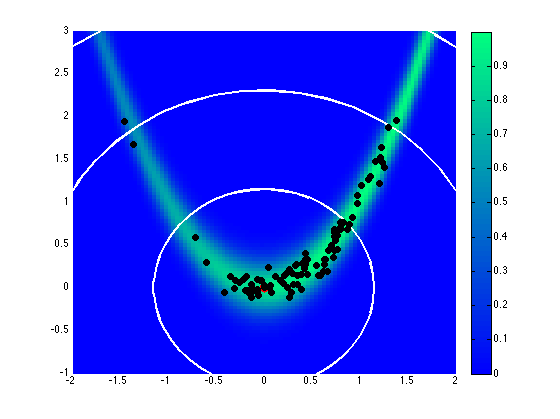
\includegraphics{images/rosen_00_prior}}
  \subfigure[Proposal covariance defined from misfit Hessian.]{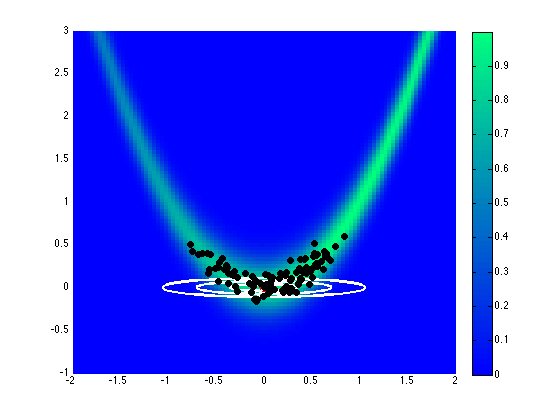
\includegraphics{images/rosen_00_pce_hessian}}
  \end{subfigmatrix}
  \caption{Depiction of proposal covariance at (0,0) with contours at one/two/three standard deviations.  2000 MCMC samples are performed and every 20th sample is plotted.}
\label{fig:rosen_prop_covar}
\end{figure}
Rejection rates for 2000 MCMC samples were 73.4\% for the former and
25.6\% for the latter.  Reducing the number of MCMC samples to 40, for
purposes of assessing local proposal accuracy, results in a similar
72.5\% rejection rate for prior-based proposal covariance and a
reduced 17.5\% rate for misfit Hessian-based proposal covariance.  The
prior-based proposal covariance only provides a global scaling and
omits information on the structure of the likelihood; as a result, the
rejection rates are relatively high for this problem and are not a
strong function of location or chain length.  The misfit Hessian-based
proposal covariance, on the other hand, provides accurate local
information on the structure of the likelihood, resulting in low
rejection rates for samples in the vicinity of this Hessian update.
Once the chain moves away from this vicinity, however, the misfit
Hessian-based approach may become inaccurate and actually impede
progress. This implies the need to regularly update a Hessian-based
proposal covariance to sustain these MCMC improvements.

In Figure~\ref{fig:rosen_restart}, we show a result for a total of
2000 MCMC samples initiated from $(-1,1)$, where we restart the chain
with an updated Hessian-based proposal covariance every 40
samples (Dakota specification: \texttt{samples = 2000
  proposal\_updates = 50}).  This case uses a standard normal prior,
resulting in differences in the MLE and MAP estimates, as shown in
Figure~\ref{fig:rosen_restart}(a).  Figure~\ref{fig:rosen_restart}(b)
shows the history of rejection rates for each of the 50 chains for
misfit Hessian-based proposals 
($\boldsymbol{\Sigma_{MVN}} = \boldsymbol{H}_{\boldsymbol{M}}^{-1}$)
and negative log posterior Hessian-based proposals 
($\boldsymbol{\Sigma_{MVN}} = \boldsymbol{H}_{\boldsymbol{\rm nlpost}}^{-1}$)
compared to the rejection rate for a single 2000-sample chain 
using prior-based proposal covariance 
($\boldsymbol{\Sigma_{MVN}} = \boldsymbol{\Sigma_0}$).
\begin{figure}[htbp]
  \begin{subfigmatrix}{2}
  \subfigure[Restarted chain.]{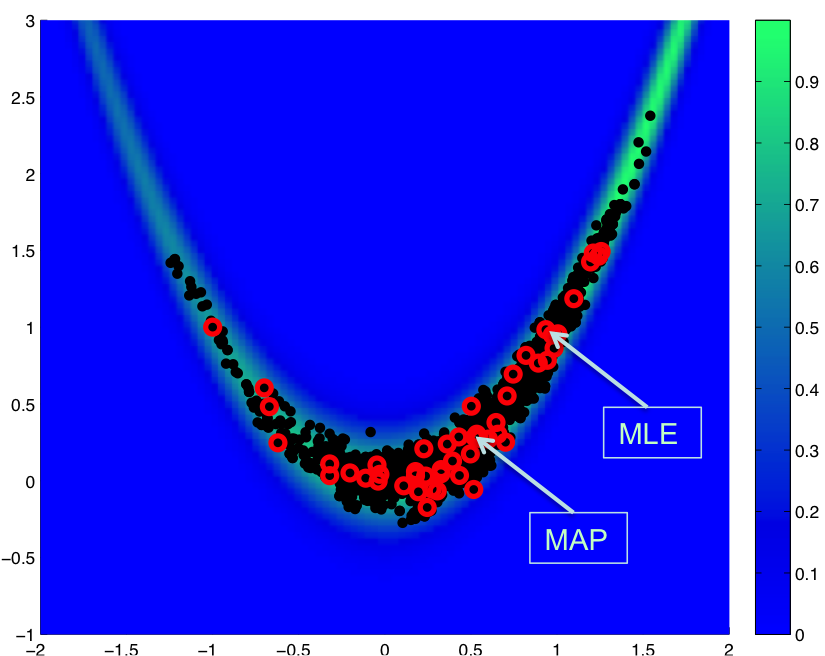
\includegraphics{images/rosen_restart_mle_map}}
  \subfigure[Rejection rates.]{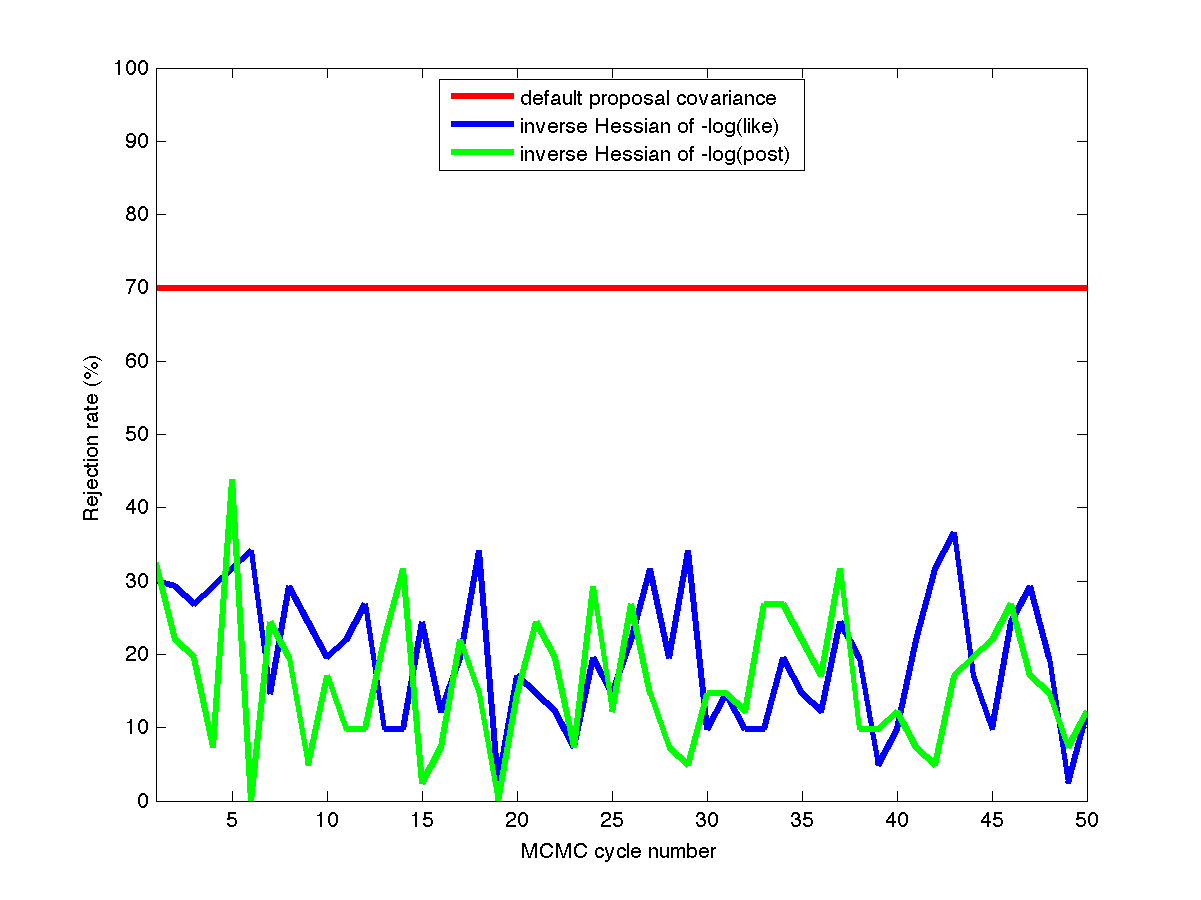
\includegraphics{images/rosen_pce_m11_50up_stdnormal_rejection}}
  \end{subfigmatrix}
  \caption{MCMC with Hessian-based proposals and standard normal prior. Left shows chain with 2000 total samples (black points) and 50 proposal updates (red circles) using the inverse of the misfit Hessian. Right shows rejection rates for misfit Hessian-based and posterior Hessian-based proposals compared to default prior covariance proposal.}
\label{fig:rosen_restart}
\end{figure}
A standard normal prior is not a strong prior in this case, and the
posterior is likelihood dominated.  This leads to similar performance
from the two Hessian-based proposals, with average rejection rates of
70\%, 19.5\%, and 16.4\% for prior-based, misfit Hessian-based, and
posterior Hessian-based cases, respectively.

\section{Model Discrepancy}\label{uq:model_disc}

Whether in a Bayesian setting or otherwise, the goal of model calibration
is to minimize the difference between the observational data $d_i$ and 
the corresponding model response $q_i(\boldsymbol{\theta})$. That is, one seeks
to minimize the misfit~\ref{eq:misfit}. For a given set of data, this 
formulation explicitly depends on model parameters that are to be adjusted and
implicitly on conditions that may vary between experiments, such as temperature
or pressure. These experimental conditions can be represented in Dakota by
configuration variables, in which case Eq.~\ref{eq:model} can be rewritten,
\begin{equation}
d_i(x) = q_i(\boldsymbol{\theta}, x) + \epsilon_i, 
\end{equation} 
where $x$ represents the configuration variables. Updated forms of the 
likelihood~\ref{eq:Likelihood} and misfit~\ref{eq:misfit} are easily obtained.

It is often the case that the calibrated model provides an insufficient fit to
the experimental data. This is generally attributed to model form or 
structural error, and can be corrected to some extent with the use of a model 
discrepancy term. The seminal work in model discrepancy techniques, Kennedy and 
O'Hagan~\cite{Kenn01} introduces an additive formulation 
\begin{equation}
d_i(x) = q_i\left(\boldsymbol{\theta}, x\right) + \delta_i(x) + \epsilon_i,
\end{equation} 
where $\delta_i(x)$ represents the model discrepancy. It should be noted and
stressed that $\delta_i$ depends \textit{only} on the configuration variables.
Future work includes expanding the model discrepancy capability in Dakota to
account for field data, so that the discrepancy may also be a function of
independent variables such as time or spacial location. Currently, one
discrepancy model is calculated for \textit{each} observable $d_i$, $i = 1, 
\ldots, n$, yielding $\delta_1, \ldots, \delta_n$.

The Dakota implementation of model discrepancy also includes the calculation
of prediction intervals for each prediction configuration $x_{k,new}$. These
intervals capture the uncertainty in the discrepancy approximation as well as
the experimental uncertainty in the response functions. It is assumed that the
uncertainties, representated by their respective variance values, are combined 
additively for each observable $i$ such that
\begin{equation}\label{eq:md_totalvar}
\Sigma_{total,i}(x) = \Sigma_{\delta,i}(x) + \sigma^2_{exp,i}(x)I,
\end{equation} 
where $\Sigma_{\delta,i}$ is the variance of the discrepancy function, and
$\sigma^2_{exp,i}$ is taken from the user-provided experimental variances.
The experimental variance provided for parameter calibration may vary for the
same observable from experiment to experiment, thus $\sigma^{2}_{exp,i}$ is
taken to be the maximum variance given for each observable. That is,
\begin{equation}
\sigma^2_{exp,i} = \max_{j} \sigma^2_{i}(x_j), 
\end{equation}
where $\sigma^2_{i}(x_j)$ is the variance provided for the $i^{th}$ observable
$d_i$, computed or measured with the configuration variable $x_j$. 
When a Gaussian process discrepancy function is used, the variance is calculated
according to Eq.~\ref{Eq:KrigVar}. For polynomial discrepancy functions, the
variance is given by Eq.~\ref{eq:poly_var}. 

%Introducing a discrepancy term gives rise to practical, as well as 
%philosphical, issues: What model form is most appropriate for $\delta_i$? How
%should $\delta_i$ be estimated? How does including $\delta_i$ change the 
%meaning or interpretation of the model responses? What is the appropriate way
%of using $\delta_i$ to improve the predictive capability of the model? 

%%add comments regarding interpolation vs extrapolation?
%kam

\subsection{Example}

For the purposes of illustrating the model discrepancy capability implemented
in Dakota, consider the following example. Let the ``truth" be given by
\begin{equation}\label{eq:md_truth}
y(t,x) = 10.5 x \log(t-0.1) - \frac{x}{(t-0.1-\theta^{*})^2},
\end{equation}
where $t$ is the independent variable, $x$ is the configuration parameter, and
$\theta^{*}$ is $7.75$, the ``true" value of the parameter $\theta$. Let the
``model" be given by
\begin{equation}\label{eq:md_model}
m(t,\theta, x) = \frac{10 x \log(t) (t-\theta)^2 - x}{(t-8)^2}. 
\end{equation}
Again, $t$ is the independent variable and $x$ is the configuration parameter,
and $\theta$ now represents the model parameter to be calibrated. It is clear
from the given formulas that the model is structurally different from the truth
and will be inadequate. 

The ``experimental" data is produced by considering two configurations, $x=10$
and $x=15$. Data points are taken over the range $t \in [1.2, 7.6]$ at 
intervals of length $\Delta t = 0.4$. Normally distributed noise $\epsilon_i$ 
is added such that
\begin{equation}\label{eq:md_data}
d_i(x_j) = y(t_i, x_j) + \epsilon_i,
\end{equation} 
with $i = 1, \ldots, 17$ and $j = 1,2$. Performing a 
Bayesian update in Dakota yields a posterior distribution of $\theta$ that is 
tightly peaked around the value $\bar{\theta} = 7.9100$. Graphs of 
$m(t, \bar{\theta}, 10)$ and $m(t, \bar{\theta}, 15)$ are compared to 
$y(t, 10)$ and $y(t, 15)$, respectively, for $t \in [1.2, 7.6]$ in 
Figure~\ref{fig:md_uncorr}, from which it is clear that the model insufficiently
captures the given experimental data.

\begin{figure}[t]
\begin{center}
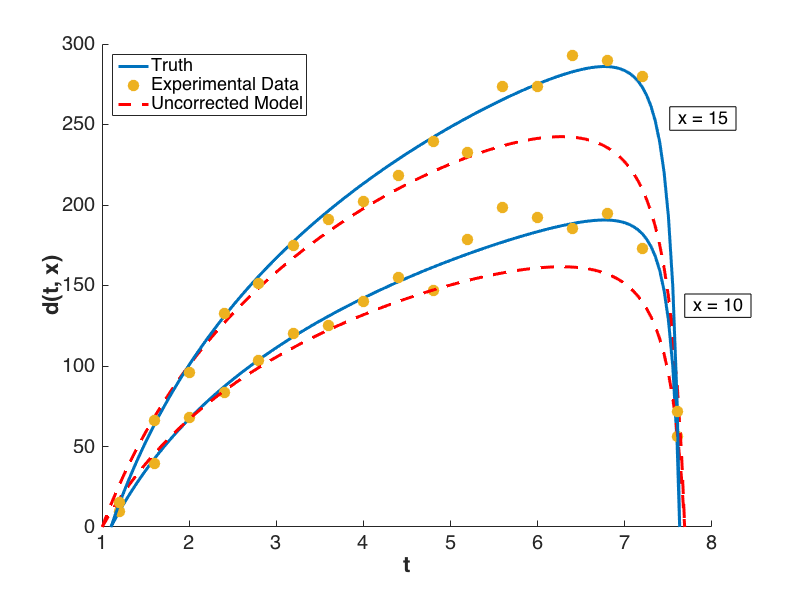
\includegraphics[width=.6\textwidth]{images/moddiscrep_TruthExpModel.png}
\end{center}
\vspace{-0.5cm}
\caption{Graphs of the uncorrected model output $m(t,x)$, the truth $y(t,x)$,
and experimental data $d(t,x)$ for configurations $x = 10$ and $x = 15$.}
\label{fig:md_uncorr}
\end{figure}

Following the Bayesian update, Dakota calculates the model discrepancy values
\begin{equation}\label{eq:md_discrep}
\delta_i(x_j) = d_i(x_j) - m_i(\bar{\theta}, x_j)
\end{equation}
for the experimental data points, \textit{i.e.}\ for $i = 1, \ldots, 17$ and
$j = 1,2$. Dakota then approximates the model discrepancy functions 
$\delta_1(x), \ldots \delta_{17}(x)$, and computes the responses and
prediction intervals of the corrected model $m_i(\bar{\theta}, x_{j,new}) 
+ \delta_i(x_{j,new})$ for each prediction configuration. The prediction
intervals have a radius of two times the standard deviation calculated 
with~\ref{eq:md_totalvar}. The discrepancy function in this example was taken
to be a Gaussian process with a quadratic trend, which is the default setting
for the model discrepancy capability in Dakota.

The prediction configurations are taken to be $x_{new} = 5, 5.5, \ldots, 20$. 
Examples of two corrected models are shown in Figure~\ref{fig:md_corr}. The
substantial overlap in the measurement error bounds and the corrected model
prediction intervals indicate that the corrected model is sufficiently accurate.
This conclusion is supported by Figure~\ref{fig:md_pred}, in which the
``truth" models for three prediction figurations are compared to the corrected
model output. In each case, the truth falls within the prediction intervals.

\begin{figure}[htbp]
\begin{center}
\subfigure[Locations of the corrected models shown in (b) and (c) below.]{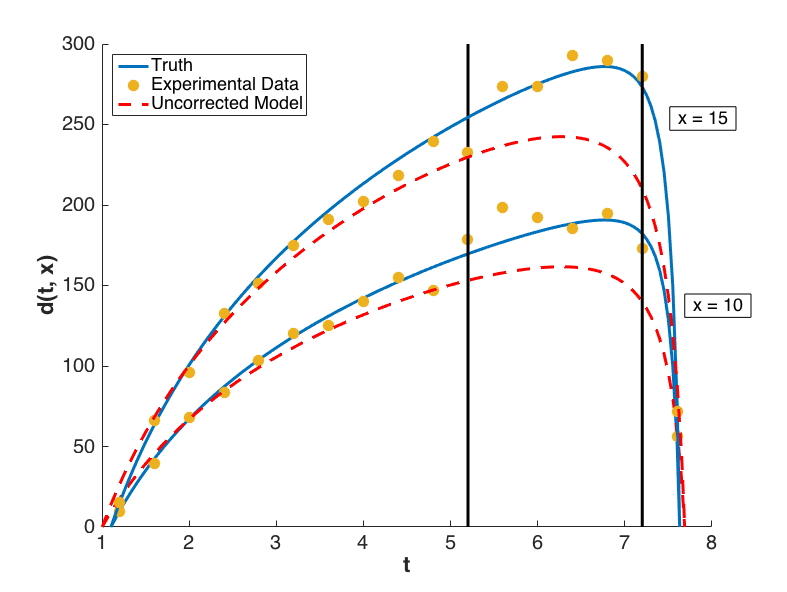
\includegraphics[width=0.6\linewidth]{images/moddiscrep_TruthExpModelGPlines.png}}
\end{center}
  \begin{subfigmatrix}{2}
  \subfigure[Corrected model values with prediction intervals for t = 5.2]{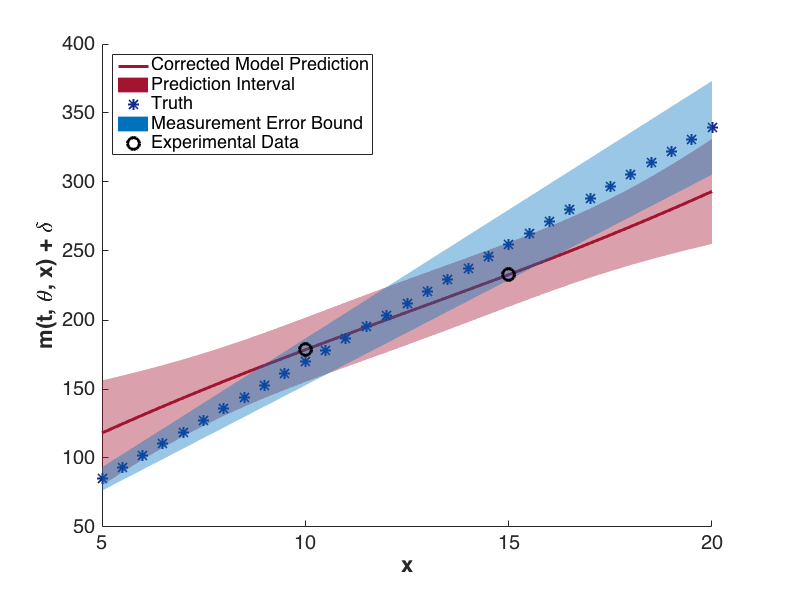
\includegraphics[width=0.49\textwidth]{images/moddiscrep_GPt5.png}}
  \subfigure[Corrected model values with prediction intervals for t = 7.2]{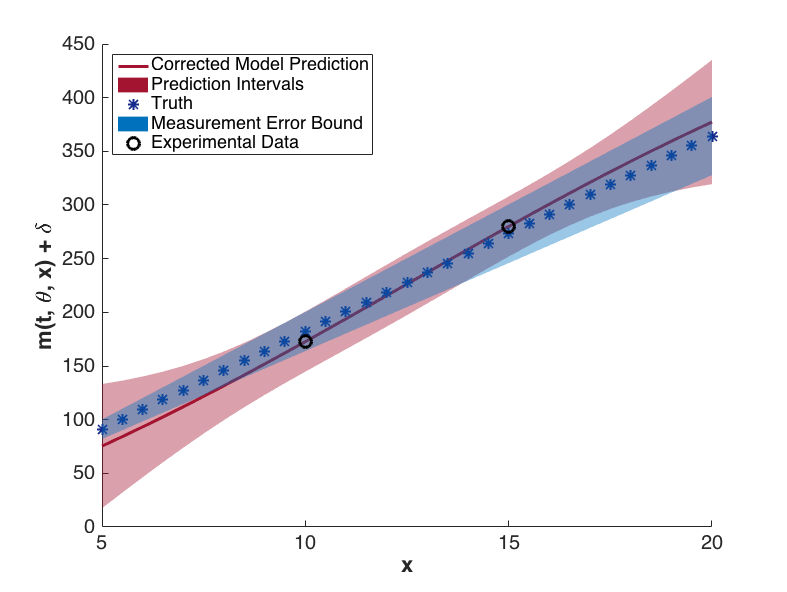
\includegraphics[width=0.49\textwidth]{images/moddiscrep_GPt7.png}}
  \end{subfigmatrix}
  \caption{Illustrated of corrected model for two observables. Note that the models shown in (b) and (c) are functions of the configuration variable $x$. Therefore, they traverse the vertical lines shown in (a).}
\label{fig:md_corr}
\end{figure}

\begin{figure}
\begin{center}
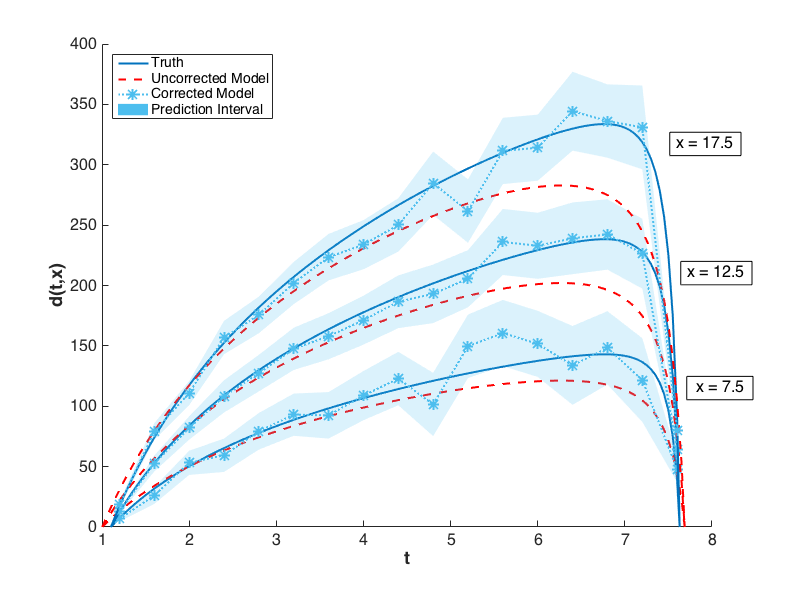
\includegraphics[width=0.6\textwidth]{images/moddiscrep_correctedlowmidhigh.png}
\end{center}
\label{fig:md_pred}
\vspace{-0.5cm}
\caption{The graphs of $y(t,x)$ for $x = 7.5, 12.5, 17.5$ are compared to the corrected model and its prediction intervals. The uncorrected model is also shown to illustrate its inadequacy.}
\end{figure}
 
\section{Experimental Design}
\label{uq:bayes_experimental_design}

Experimental design algorithms seek to add observational data that informs
model parameters and reduces their uncertainties. Typically, the observational 
data $\boldsymbol{d}$ used in the Bayesian update~\ref{eq:BayesThm} is taken
from physical experiments. However, it is also common to use the responses or
output from a high-fidelity model as $\boldsymbol{d}$ in the calibration of a
low-fidelity model. Furthermore, this calibration can be done with a single
Bayesian update or iteratively with the use of experimental design. The context
of experimental design mandates that the high-fidelity model or physical 
experiment depend on design conditions or configurations, such as temperature
or spatial location. After a preliminary Bayesian update using an initial set 
of high-fidelity (or experimental) data, the next ``best" design points are 
determined and used in the high-fidelity model to augment 
$\boldsymbol{d}$, which is used in subsequent Bayesian updates of the 
low-fidelity model parameters.

The question then becomes one of determining the meaning of ``best." In 
information theory, the mutual information is a measure of the reduction in the 
uncertainty of one random variable due to the knowledge of 
another~\cite{Cov2006}. Recast into the context of experimental design, the 
mutual information represents how much the proposed experiment and resulting 
observation would reduce the uncertainties in the model parameters. Therefore, 
given a set of experimental design conditions, that which maximizes the mutual 
information is the most desirable. This is the premise that motivates the 
Bayesian experimental design algorithm implemented in Dakota.

The initial set of high-fidelity data may be either user-specified or generated
within Dakota by performing Latin Hypercube Sampling on the space of 
configuration variables specified in the input file. If Dakota-generated, the 
design variables will be run through the high-fidelity model specified by the
user to produce the initial data set. Whether user-specified or 
Dakota-generated, this initial data is used in a Bayesian update of the 
low-fidelity model parameters. 

It is important to note that the low-fidelity model depends on both parameters 
to be calibrated $\boldsymbol{\theta}$ and the design conditions 
$\boldsymbol{\xi}$. During Bayesian calibration, $\boldsymbol{\xi}$ are not 
calibrated; they do, however, play an integral role in the calculation of the 
likelihood. Let us rewrite Bayes' Rule as
\begin{equation}
{f_{\boldsymbol{\Theta |D}}}\left( \boldsymbol{\theta |d(\xi)} \right) 
= \frac{{{f_{\boldsymbol{\Theta}}}\left( \boldsymbol{\theta} \right)
\mathcal{L}\left( \boldsymbol{\theta;d(\xi)} \right)}}
{{{f_{\boldsymbol{D}}}\left( \boldsymbol{d(\xi)} \right)}},
\label{eq:expdesign_bayes}
\end{equation}
making explicit the dependence of the data on the design conditions. As in
Section~\ref{uq:bayes:basic}, the difference between the high-fidelity and 
low-fidelity model responses is assumed to be Gaussian such that
\begin{equation}
d_{i}(\boldsymbol{\xi_{j}}) = q_{i}(\boldsymbol{\theta,\xi}_{j}) + \epsilon_{i},
\end{equation}
where $\boldsymbol{\xi}_{j}$ are the configuration specifications of the $j$th 
experiment. The experiments are considered to be independent, making the misfit 
\begin{equation}
M(\boldsymbol{\theta, d(\xi)}) = \frac{1}{2} \sum_{j = 1}^{m} 
\left( \boldsymbol{d}(\boldsymbol{\xi}_{j}) - 
\boldsymbol{q}(\boldsymbol{\theta, \xi}_{j}) \right)^{T}
\boldsymbol{\Sigma}_{\boldsymbol{d}}^{-1}
\left( \boldsymbol{d}(\boldsymbol{\xi}_{j}) - 
\boldsymbol{q}(\boldsymbol{\theta, \xi}_{j}) \right).
\end{equation}

At the conclusion of the initial calibration, a set of candidate design
conditions is proposed. As before, these may be either user-specified or
generated within Dakota via Latin Hypercube Sampling of the design space. Among
these candidates, we seek that which maximizes the mutual information,
\begin{equation}
\boldsymbol{\xi}^{*} = \argmax_{\boldsymbol{\xi}_{j}} I(\boldsymbol{\theta},
\boldsymbol{d}(\boldsymbol{\xi}_{j}) ),
\label{eq:optimal_design}
\end{equation}
where the mutual information is given by
\begin{equation}
I(\boldsymbol{\theta}, \boldsymbol{d}(\boldsymbol{\xi}_{j})) = \iint 
{f_{\boldsymbol{\Theta ,D}}}\left( \boldsymbol{\theta ,d(\xi}_{j}) \right)
\log \frac{ {f_{\boldsymbol{\Theta,D}}}\left( \boldsymbol{\theta,d(\xi}_{j}) 
\right)}{f_{\boldsymbol{\Theta}}\left(\boldsymbol{\theta} \right) 
f_{\boldsymbol{D}}\left(\boldsymbol{d}(\boldsymbol{\xi}_{j}) \right) }
d\boldsymbol{\theta} d\boldsymbol{d}.
\label{eq:mutual_info}
\end{equation}

The mutual information must, therefore, be computed for each candidate design 
point $\boldsymbol{\xi}_{j}$. There are two $k$-nearest neighbor methods 
available in Dakota that can be used to approximate Eq.~\ref{eq:mutual_info}, 
both of which are derived in~\cite{Kra04}. Within Dakota, the posterior 
distribution 
$f_{\boldsymbol{\Theta | D}}\left(\boldsymbol{\theta | d(\xi)}\right)$ is given
by MCMC samples. From these, $N$ samples are drawn and run through the
low-fidelity model with $\boldsymbol{\xi}_{j}$ fixed. This creates a matrix 
whose rows consist of the vector $\boldsymbol{\theta}^{i}$ and the low-fidelity
model responses $\tilde{\boldsymbol{d}}(\boldsymbol{\theta}^{i}, 
\boldsymbol{\xi}_{j})$ for $i = 1, \ldots, N$. These rows 
represent the joint distribution between the parameters and model responses. 
For each row $X_{i}$, the distance to its $k^{th}$-nearest neighbor among the 
other rows is approximated $\varepsilon_{i} = \| X_{i} - X_{k(i)} \|_{\infty}$. 
As noted in~\cite{Lew16}, $k$ is often taken to be six. The treatment of the 
marginal distributions is where the two mutual information algorithms differ. 
In the first algorithm, the marginal distributions are considered by 
calculating $n_{\boldsymbol{\theta},i}$, which is the number of parameter 
samples that lie within $\varepsilon_{i}$ of $\boldsymbol{\theta}^{i}$, and 
$n_{\boldsymbol{d},i}$, which is the number of responses that lie within 
$\varepsilon_{i}$ of $\tilde{\boldsymbol{d}}(\boldsymbol{\theta}^{i}, 
\boldsymbol{\xi}_{j})$. The mutual information then is approximated 
as~\cite{Kra04}
\begin{equation}
\label{eq:ksg1}
I(\boldsymbol{\theta}, \boldsymbol{d}(\boldsymbol{\xi}_{j})) \approx
\psi(k) + \psi(N) - \frac{1}{N-1} \sum_{i = 1}^{N} \left[ 
\psi(n_{\boldsymbol{\theta},i}) - \psi(n_{\boldsymbol{d},i}) \right],
\end{equation}
where $\psi(\cdot)$ is the digamma function. 

In the second mutual information approximation method, $X_{i}$ and all of 
its $k$-nearest neighbors such that $\| X_{i} - X_{l} \|_{\infty} < 
\varepsilon_{i}$ are projected into the marginal subspaces for 
$\boldsymbol{\theta}$ and $\tilde{\boldsymbol{d}}$. The quantity 
$\varepsilon_{\boldsymbol{\theta},i}$ is then defined as the radius of the 
$l_{\infty}$-ball containing all $k+1$ projected values of 
$\boldsymbol{\theta}_{l}$. Similarly, $\varepsilon_{\boldsymbol{d},i}$ is 
defined as the radius of the $l_{\infty}$-ball containing all $k+1$ projected 
values of $\tilde{\boldsymbol{d}}(\boldsymbol{\theta}_{l}, 
\boldsymbol{\xi}_{j})$~\cite{Gao14}. In this version of the mutual information 
calculation, $n_{\boldsymbol{\theta},i}$ is the number of parameter samples 
that lie within $\varepsilon_{\boldsymbol{\theta},i}$ of 
$\boldsymbol{\theta}^{i}$, and $n_{\boldsymbol{d},i}$ is the number of 
responses that lie within $\varepsilon_{\boldsymbol{d}, i}$ of 
$\tilde{\boldsymbol{d}}(\boldsymbol{\theta}^{i}, \boldsymbol{\xi}_{j})$. 
The mutual information then is approximated as~\cite{Kra04}
\begin{equation}
\label{eq:ksg2}
I(\boldsymbol{\theta}, \boldsymbol{d}(\boldsymbol{\xi}_{j})) \approx
\psi(k) + \psi(N) - \frac{1}{k} - \frac{1}{N-1} \sum_{i = 1}^{N} \left[ 
\psi(n_{\boldsymbol{\theta},i}) - \psi(n_{\boldsymbol{d},i}) \right].
\end{equation}

By default, Dakota uses Eq.~\ref{eq:ksg1} to approximate the mutual
information. The user may decide to use Eq.~\ref{eq:ksg2} by including the
keyword \texttt{ksg2} in the Dakota input script. An example can be found 
in~\cite{RefMan}. Users also have the option of specifying statistical noise
in the low-fidelity model through the \texttt{simulation\_variance} keyword.
When this option is included in the Dakota input file, a random ``error" is
added to the low-fidelity model responses when the matrix $X$ is built. This
random error is normally distributed, with variance equal to
\texttt{simulation\_variance}.

Once the optimal design $\boldsymbol{\xi}^{*}$ is identified, it is run 
through the high-fidelity model to produce a new data point $\boldsymbol{d}(
\boldsymbol{\xi}^{*})$, which is added to the calibration data. Theoretically,
the current posterior $f_{\boldsymbol{\Theta | D}}\left(\boldsymbol{\theta | 
d(\xi)}\right)$ would become the prior in the new Bayesian update, and the 
misfit would compare the low-fidelity model output \textit{only} to the new
data point. However, as previously mentioned, we do not have the posterior
distribution; we merely have a set of samples of it. Thus, each time the set
of data is modified, the \textit{user-specified} prior distribution is used
and a full Bayesian update is performed from scratch. If none of the three
stopping criteria is met, $\boldsymbol{\xi}^{*}$ is removed from the set of
candidate points, and the mutual information is approximated for those that
remain using the newly updated parameters. These stopping criteria are:
\begin{itemize}
\item the user-specified maximum number of high-fidelity model evaluations is 
reached (this does not include those needed to create the initial 
data set)
\item the relative change in mutual information from one iteration to the next
is sufficiently small (less than $5\%$)
\item the set of proposed candidate design conditions has been exhausted
\end{itemize}
If any one of these criteria is met, the algorithm is considered complete.

\subsection{Batch Point Selection}

The details of the experimental design algorithm above assume only one
optimal design point is being selected for each iteration of the algorithm.
The user may specify the number of optimal design points to be
concurrently selected by including the \texttt{batch\_size} in the input
script. The optimality condition~\ref{eq:optimal_design} is then replaced by
\begin{equation}
\left\{ \boldsymbol{\xi}^{*} \right\} = \argmax I\left(\boldsymbol{\theta}, 
\left\{ \boldsymbol{d}(\boldsymbol{\xi})\right\}\right),
\label{eq:batch_xi_true}
\end{equation} 
where $\left\{ \boldsymbol{\xi}^{*} \right\} = \left\{ \boldsymbol{\xi}^{*}_{1},
\boldsymbol{\xi}_{2}^{*}, \ldots, \boldsymbol{\xi}_{s}^{*} \right\}$ is the 
set of optimal designs, $s$ being defined by \texttt{batch\_size}. If the set
of design points from which the optimal designs are selected is of size $m$,
finding $\left\{ \boldsymbol{\xi}^{*} \right\}$ as in~\ref{eq:batch_xi_true}
would require $m!/(m-s)!$ mutual information calculations, which may become
quite costly. Dakota therefore implements a greedy batch point selection
algorithm in which the first optimal design,
\begin{equation}
\boldsymbol{\xi}^{*}_{1} = \argmax_{\boldsymbol{\xi}_{j}} I(\boldsymbol{\theta},
\boldsymbol{d}(\boldsymbol{\xi}_{j}) ),
\end{equation} 
is identified, and then used to find the second,
\begin{equation}
\boldsymbol{\xi}^{*}_{2} = \argmax_{\boldsymbol{\xi}_{j}} 
I(\boldsymbol{\theta}, \boldsymbol{d}(\boldsymbol{\xi}_{j}) |
\boldsymbol{d}(\boldsymbol{\xi}_{1}^{*})).
\end{equation} 
Generally, the $i^{th}$ selected design will satisfy
\begin{equation}
\boldsymbol{\xi}^{*}_{i} = \argmax_{\boldsymbol{\xi}_{j}} 
I(\boldsymbol{\theta}, \boldsymbol{d}(\boldsymbol{\xi}_{j}) |
\boldsymbol{d}(\boldsymbol{\xi}_{1}^{*}), \ldots, 
\boldsymbol{d}(\boldsymbol{\xi}_{i-1}^{*})).
\end{equation} 

The same mutual information calculation algorithms~\ref{eq:ksg1} 
and~\ref{eq:ksg2} described above are applied when calculating the conditional
mutual information. The additional low-fidelity model information is 
appended to the responses portion of the matrix $X$, and the calculation of
$\varepsilon_{i}$ or $\varepsilon_{\boldsymbol{d}, i}$ as well as 
$n_{\boldsymbol{d}, i}$ are adjusted accordingly.  

\section{Information Theoretic Tools}\label{uq:info_theory}

The notion of the entropy of a random variable was introduced by C.E. 
Shannon in 1948~\cite{Sha1948}. So named for its resemblance to the statistical 
mechanical entropy, the Shannon entropy (or simply the entropy), is 
characterized by the probability distribution of the random variable being 
investigated. For a random variable $X \in \mathcal{X}$ with probability 
distribution function $p$, the entropy $h$ is given by
\begin{equation}
h(p) = -\int_{\mathcal{X}} p(x) \log p(x) dx.
\label{ent_cont}
\end{equation}
The entropy captures the average uncertainty in a random 
variable~\cite{Cov2006}, and is therefore quite commonly used in predictive 
science. The entropy also provides the basis for other information measures, 
such as the relative entropy and the mutual information, both of which compare 
the information content between two random variables but have different 
purposes and interpretations. 

The relative entropy provides a measure of the difference between two 
probability distributions. It is characterized by the Kullback-Leibler 
Divergence,
\begin{equation}
D_{KL}(p \| q) = \int p(x) \log \frac{p(x)}{q(x)} dx,
\label{dkl_discrete}
\end{equation}
which can also be written as 
\begin{equation}
D_{KL}( p \| q)  = h(p,q) - h(p),
\end{equation}
where $h(p,q)$ is the cross entropy of two distributions,
\begin{equation}
h(p,q) = \int p(x) \log q(x) dx.
\end{equation}
Because it is not symmetric ($D_{KL} (p \| q) \neq D_{KL} (q \| p)$), the 
Kullback-Leibler Divergence is sometimes referred to as a pseudo-metric. 
However, it is non-negative, and equals zero if and only if $p = q$. 

As in Section~\ref{uq:bayes_experimental_design}, the Kullback-Leibler 
Divergence is approximated with the $k$-nearest neighbor method advocated 
in~\cite{Per2008}. Let the distributions $p$ and $q$ be represented by a 
collection of samples of size $n$ and $m$, respectively. For each sample $x_{i}$
in $p$, let $\nu_{k}(i)$ be the distance to it's $k^{th}$-nearest neighbor among
the remaining samples of $p$. Furthermore, let $\rho_{k}(i)$ be the distance 
between $x_{i}$ and its $k^{th}$-nearest neighbor among the samples of $q$. If 
either of these distances is zero, the first non-zero neighbor distance is 
found, yielding a more general notation: $\nu_{k_i}(i)$ and $\rho_{l_i}(i)$, 
where $k_{i}$ and $l_{i}$ are the new neighbor counts and are greather than or 
equal to $k$. Then 
\begin{equation}
D_{KL}(p \| q) \approx \frac{d}{n} \sum_{i=1}^{n} \left[ \log \frac{
\nu_{k_{i}}(i)}{\rho_{l_{i}}(i)} \right] + \frac{1}{n} \sum_{i=1}^{n} 
\left[ \psi(l_{i}) - \psi(k_{i}) \right] + \log \frac{m}{n-1},
\end{equation}
where $\psi(\cdot)$ is the digamma function. In Dakota, $k$ is taken to be six.

The Kullback-Leibler Divergence is used within Dakota to quantify the amount of
information gained during Bayesian calibration,
\begin{equation}
IG( f_{\boldsymbol{\Theta | D}}(\boldsymbol{\theta| d}); 
f_{\boldsymbol{\Theta}}(\boldsymbol{\theta}))
= D_{KL}( f_{\boldsymbol{\Theta | D}}(\boldsymbol{\theta| d}) \| 
f_{\boldsymbol{\Theta}}(\boldsymbol{\theta}) ). 
\end{equation}
If specified in the input file, the approximate value will be output to the
screen at the end of the calibration.

In the presence of two (possibly multi-variate) random variables, the mutual 
information quantifies how much information they contain about each other. In 
this sense, it is a measure of the mutual dependence of two random variables. 
For continuous $X$ and $Y$, 
\begin{equation}
I(X, Y) = \iint p(x,y) \log \frac{ p(x,y) }{p(x)p(y)} \; dx \, dy,
\end{equation}
where $p(x,y)$ is the joint pdf of $X$ and $Y$, while $p(x)$ and $p(y)$ are the 
marginal pdfs of $X$ and $Y$, respectively. The mutual information is symmetric 
and non-negative, with zero indicating the independence of $X$ and $Y$. It is 
related to the Kullback-Leibler Divergence through the expression
\begin{equation}
I(X,Y) = D_{KL} ( p(x,y) \| p(x) p(y) ). 
\end{equation}
The uses of the mutual information within Dakota have been noted in 
Section~\ref{uq:bayes_experimental_design}.



\section{Measure-theoretic Stochastic Inversion} \label{uq:cbayes}

% MACROS FOR THIS SECTION
\newcommand{\pspace}{\mathbf{\Lambda}}
\newcommand{\dspace}{\mathbf{\mathcal{D}}}
\newcommand{\pmeas}{\mu_{\pspace}}
\newcommand{\dmeas}{\mu_{\dspace}}
\newcommand{\pborel}{\mathcal{B}_{\pspace}}
\newcommand{\dborel}{\mathcal{B}_{\dspace}}
\newcommand{\priormeas}{P_{\pspace}^{\text{prior}}}
\newcommand{\postmeas}{P_{\pspace}^{\text{post}}}
\newcommand{\priordens}{\pi_{\pspace}^{\text{prior}}}
\newcommand{\postdens}{\pi_{\pspace}^{\text{post}}}
\newcommand{\pfpriormeas}{P_{\dspace}^{Q(\text{prior})}}
\newcommand{\pfpostmeas}{P_{\dspace}^{Q(\text{post})}}
\newcommand{\pfpriordens}{\pi_{\dspace}^{Q(\text{prior})}}
\newcommand{\pfpostdens}{\pi_{\dspace}^{Q(\text{post})}}
\newcommand{\obsmeas}{P_{\dspace}^{\text{obs}}}
\newcommand{\obsdens}{\pi_{\dspace}^{\text{obs}}}
\newcommand{\postdenssbayes}{\tilde{\pi}_{\pspace}^{\text{post}}}


In this section we present an overview of a specific implementation of the measure-theoretic approach for solving a stochastic inverse problem
that incorporates prior information and Bayes' rule to define a unique solution.
This approach differs from the standard Bayesian counterpart described in previous sections in that the posterior satisfies a consistency requirement with the model and the observed data.
The material in this section is based on the foundational work in \cite{Butler2017, Walsh2017}.
A more thorough description of this consistent Bayesian approach and a comparison with the standard Bayesian approach can be found in \cite{Butler2017} and an extension to solve an optimal experimental design problem can be found in \cite{Walsh2017}.

Let $M(Y,\lambda)$ denote a deterministic model with solution $Y(\lambda)$ that is an implicit function of model parameters $\lambda\in\pspace \subset \mathbb{R}^n$.
The set $\pspace$ represents the largest physically meaningful domain of parameter values, and, for simplicity, we assume that $\pspace$ is compact.
We assume we are only concerned with computing  a relatively small set of quantities of interest (QoI), $\{Q_i(Y)\}_{i=1}^m$, where each $Q_i$ is a real-valued functional dependent on the model solution $Y$.
Since $Y$ is a function of parameters $\lambda$, so are the QoI and we write $Q_i(\lambda)$ to make this dependence explicit.
Given a set of QoI, we define the QoI map $Q(\lambda) := (Q_1(\lambda), \cdots, Q_m(\lambda))^\top:\pspace\to\dspace\subset\mathbb{R}^m$ where $\dspace  := Q(\pspace)$ denotes the range of the QoI map.

We assume $(\pspace, \pborel, \pmeas)$ and $(\dspace, \dborel, \dmeas)$ are measure spaces
and let $\pborel$ and $\dborel$ denote the Borel $\sigma$-algebras inherited from the metric topologies on $\mathbb{R}^n$ and $\mathbb{R}^m$, respectively.
We also assume that the QoI map $Q$ is at least piecewise smooth implying that $Q$ is a measurable map between the measurable spaces $(\pspace, \pborel)$ and $(\dspace, \dborel)$.
For any $A\in\dborel$, we then have
\[Q^{-1}(A) = \left\{ \lambda \in \pspace \ | \ Q(\lambda) \in A \right\}\in\pborel, \quad \text{and} \quad Q(Q^{-1}(A))=A.\]
Furthermore, given any $B\in\pborel$,
\begin{equation}\label{:eq:mapprops}
B \subseteq Q^{-1}(Q(B)),
\end{equation}
although we note that in most cases $B\neq Q^{-1}(Q(B))$ even when $n=m$.

Finally, we assume that an observed probability measure, $\obsmeas$, is given on $(\dspace,\dborel)$, and the stochastic inverse problem seeks a probability measure $P_\pspace$
such that the subsequent push-forward measure induced by the map, $Q(\lambda)$, satisfies
\begin{equation}\label{:eq:invdefn}
P_\pspace(Q^{-1}(A)) = P^{Q(P_\pspace)}_\dspace(A) = \obsmeas(A),
\end{equation}
for any $A\in \dborel$.

This inverse problem may not have a unique solution, i.e., there
may be multiple probability measures that have the proper push-forward measure.
A unique solution may be obtained by imposing additional constraints or structure on the stochastic inverse problem.
The approach we consider in this section incorporates prior information and Bayes rule to construct a unique
solution to the stochastic inverse problem.
The prior probability measure and the map
induce a push-forward measure $\pfpriormeas$ on $\dspace$, which is defined for all $A\in \dborel$,
\begin{equation}\label{:eq:pfprior}
\pfpriormeas(A) = \priormeas(Q^{-1}(A)).
\end{equation}

We assume that all of the probability measures (prior, observed and push-forward of the prior) are absolutely continuous with respect to some reference measure
and can be described in terms of a probability densities.
We use $\priordens$, $\obsdens$ and $\pfpriordens$ to denote the probability densities associated
with $\priormeas$, $\obsmeas$ and $\pfpriormeas$ respectively.
From \cite{Butler2017}, the following posterior probability density, when interpreted through a disintegration theorem, solves the stochastic inverse problem:
\begin{equation}\label{:eq:postpdf}
\postdens(\lambda) = \priordens(\lambda)\frac{\obsdens(Q(\lambda))}{\pfpriordens(Q(\lambda))}, \quad \lambda \in \pspace.
\end{equation}
One can immediately observe that if $\pfpriordens = \obsdens$, i.e., if the prior solves the stochastic inverse problem in the sense that the push-forward of the prior matches the observations,
then the posterior will be equal to the prior.
Approximating this posterior density requires an approximation
of the push-forward of the prior, which is simply a forward
propagation of uncertainty.
